% Copyright 2004 by Till Tantau <tantau@users.sourceforge.net>.
%
% In principle, this file can be redistributed and/or modified under
% the terms of the GNU Public License, version 2.
%
% However, this file is supposed to be a template to be modified
% for your own needs. For this reason, if you use this file as a
% template and not specifically distribute it as part of a another
% package/program, I grant the extra permission to freely copy and
% modify this file as you see fit and even to delete this copyright
% notice. 
\UseRawInputEncoding
\documentclass{beamer}

% There are many different themes available for Beamer. A comprehensive
% list with examples is given here:
% http://deic.uab.es/~iblanes/beamer_gallery/index_by_theme.html
% You can uncomment the themes below if you would like to use a different
% one:
%\usetheme{AnnArbor}
%\usetheme{Antibes}
%\usetheme{Bergen}
%\usetheme{Berkeley}
%\usetheme{Berlin}
%\usetheme{Boadilla}
%\usetheme{boxes}
%\usetheme{CambridgeUS}
%\usetheme{Copenhagen}
%\usetheme{Darmstadt}
%\usetheme{default}
%\usetheme{Frankfurt}
%\usetheme{Goettingen}
%\usetheme{Hannover}
%\usetheme{Ilmenau}
%\usetheme{JuanLesPins}
%\usetheme{Luebeck}
\usetheme{Madrid}
%\usetheme{Malmoe}
%\usetheme{Marburg}
%\usetheme{Montpellier}
%\usetheme{PaloAlto}
%\usetheme{Pittsburgh}
%\usetheme{Rochester}
%\usetheme{Singapore}
%\usetheme{Szeged}
%\usetheme{Warsaw}

\usepackage{pgfgantt}
%\usepackage{todonotes}
\usepackage{media9}
\usepackage{subfigure}


% Customize Warsaw color 
\setbeamercolor*{palette primary}{use=structure,fg=white,bg=blue!50!black}
\setbeamercolor*{palette secondary}{use=structure,fg=white,bg=blue!60!black}
\setbeamercolor*{palette tertiary}{use=structure,fg=white,bg=blue!70!black}

% Customize Warsaw block title and background colors
\setbeamercolor{block title}{bg=red!50!black,fg=white}

\setbeamertemplate{bibliography item}{\insertbiblabel}  % insert bibliography numbers instead of symbol
\setbeamertemplate{caption}[numbered] % adds the figure or table number to the caption.



\title[Project Proposal]{Senior Capstone Project I\\\textbf{\underline{Project Proposal}}\\
\vspace{0.25in}
Project Title: Development of an Intelligent Building Energy Management Platform}

% % A subtitle is optional and this may be deleted
% \subtitle{Product Proposal}

\author[B.~Lauer, E.~Watkins]{Brian~Lauer \and Elliot~Watkins \and
Advisor: Dr. Suruz Miah}
% - Give the names in the same order as the appear in the paper.
% - Use the \inst{?} command only if the authors have different
%   affiliation.

\institute[Bradley University] % (optional, but mostly needed)
{
  Department of Electrical and Computer Engineering\\
  Bradley University\\
  1501 W. Bradley Avenue\\
  Peoria, IL, 61625, USA
}
% - Use the \inst command only if there are several affiliations.
% - Keep it simple, no one is interested in your street address.

%\date[November~27,~2018]{Tuesday, November~27,~2018}
\date[November~30,~2020]{Monday, November~30,~2020}
%\date[December~4,~2018]{Tuesday, December~4,~2016}

% - Either use conference name or its abbreviation.
% - Not really informative to the audience, more for people (including
%   yourself) who are reading the slides online

\logo{\hfill\href{http://www.bradley.edu}{
\includegraphics[width=0.75cm]{figs/logoBU1-Print}}}  % place logo in every page 

\subject{Building Energy Management}
% This is only inserted into the PDF information catalog. Can be left
% out. 

% If you have a file called "university-logo-filename.xxx", where xxx
% is a graphic format that can be processed by latex or pdflatex,
% resp., then you can add a logo as follows:

% \pgfdeclareimage[height=0.5cm]{university-logo}{university-logo-filename}
% \logo{\pgfuseimage{university-logo}}

% Delete this, if you do not want the table of contents to pop up at
% the beginning of each subsection:
\AtBeginSubsection[]
{
  \begin{frame}<beamer>{Outline}
    \tableofcontents[currentsection,currentsubsection]
  \end{frame}
}

% Let's get started
\begin{document}

\begin{frame}
  \titlepage
\end{frame}

\begin{frame}{Outline} %
  \tableofcontents%[pausesections]
  % You might wish to add the option [pausesections]
\end{frame}

% Section and subsections will appear in the presentation overview
% and table of contents.
\section{Introduction}
%\section{Project Description}
\section{Background Study}
\section{Functional Requirements}
\section{System Architecture}
\section{Preliminary Work}
\section{Parts List}
\section{Timeline and Milestones}

\begin{frame}{Introduction}{}
    % High-Level Architecture Figure
    \begin{figure}
        \centering
        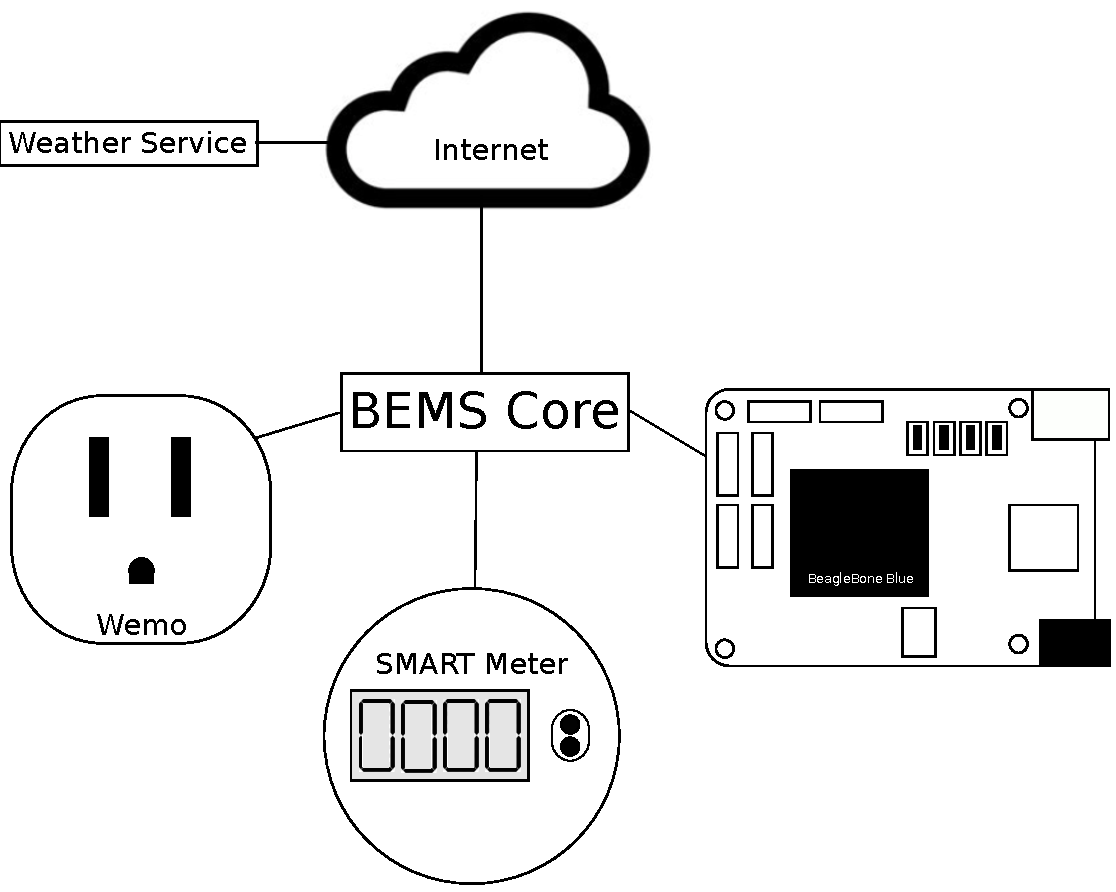
\includegraphics[scale=0.4]{figs/highLevelArchitecture.pdf}
        \caption{High level architecture}
        \label{fig:my_label}
    \end{figure}
\end{frame}

\begin{frame}{Introduction}{}
    % Applications of Building Energy Management
    \begin{itemize}
        \item BEMS Core will interface with as many devices as it has support for 
        \begin{itemize}
            \item Wemo and Embedded Computer will be fully functional by end of semester
            \item User will be able to control these devices directly from the Web Server
        \end{itemize}
        \item In the Spring, we hope to simulate a microgrid with MATLAB Simscape and an HVAC System with Simulink
        \begin{itemize}
            \item The microgrid simulation will allow us to virtually measure a power meter
            \item An HVAC System in Simulink could be controlled with a Linear Quadratic Regulator (LQR) based algorithm that can regulate the building temperature
        \end{itemize}
        \item If time allows, we will also have the BEMS Core ping a weather service for updates on severe weather as well
    \end{itemize}
\end{frame}

\begin{frame}{Background Study}{}
    \begin{itemize} % Break down more (talk about BEMOSS possibly) and the LoBEMS project
        \item An existing BEMS described in~\cite{Mataloto2019} incorporates its own sensors for:
        \begin{itemize}
            \item temperature
            \item humidity
            \item luminosity
            \item air quality
            \item motion
        \end{itemize}
        \item The data from these sensors is fed to the BEMS core where decisions are made for the HVAC system and lighting of the building
        \item While we will only be simulating HVAC with Simscape, our BEMS core is similar to this project in that we are using IoT as a communication platform
    \end{itemize}
\end{frame}

\begin{frame}{Background Study}{}
\begin{itemize}
    \item MPC (Model Predictive Control) used in~\cite{Mayer2017} 
    \item Building control split into two levels for building automation improvement
    \item Examples of the usage of MPC given are temperature control and interaction with smart grids
\end{itemize}    
\end{frame}

\begin{frame}{Background Study}{}
\begin{figure}
    \centering
    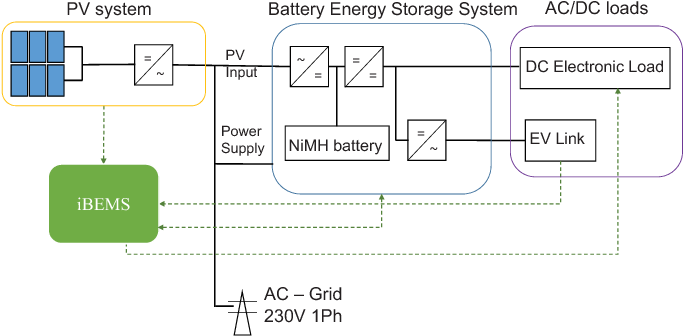
\includegraphics[scale=0.45]{figs/img/pvBESSystem.png}
    \caption{Photovoltaic (Battery Energy Storage) BES system simulated in \cite{Barchi2018}}
    \label{fig:pvBESSystem}
\end{figure}
\end{frame}

\begin{frame}{Functional Requirements}{}
    \begin{itemize}
        \item The minimum viable product will be to connect to a Wemo Insight Smart Plug and a Embedded Computer (BeagleBone Blue)
        \begin{itemize}
            \item The WeMo Plug will simply be turned on and off from the Web Server. The BEMS Core will also record its power usage
            \item The only functionality needed on the BeagleBone Blue will be PWM input to the motor drivers
        \end{itemize}
        \item A database (Apache Cassandra) will be implemented for recording power usage
    \end{itemize}
\end{frame}

\begin{frame}{System Architecture}{}
    % Functional Block Diagram
    \begin{figure}
        \centering
        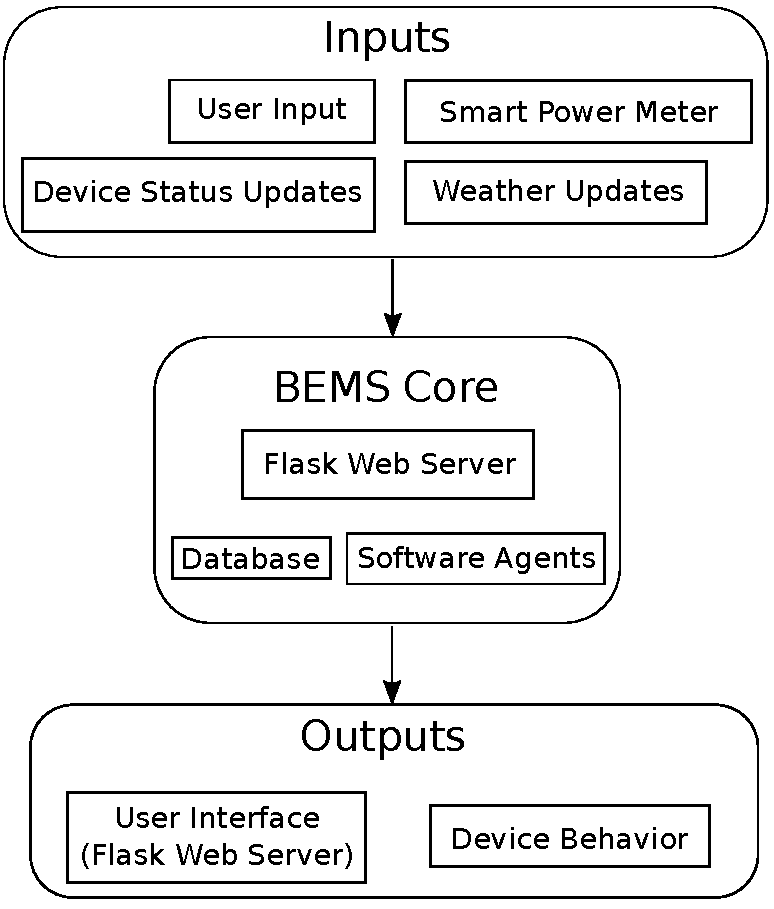
\includegraphics[scale=0.4]{figs/functionalBlockDiagram.pdf}
        \caption{Functional block diagram of the BEMS}
        \label{fig:my_label}
    \end{figure}
\end{frame}

\begin{frame}{System Architecture - Inputs}{}
    % What are we using to build this?
    \begin{itemize}
        \item Users
            \begin{itemize}
                \item Adjust the operation of a device (turn up the temperature of an AC unit, for instance)
                \item Turn a device on or off
            \end{itemize}
        \item Smart power meters will be able to connect the platform and give real-time updates of the building's overall power usage
        \item Connected Devices
            \begin{itemize}
                \item The Wemo Switch and Embedded Computer will have master-slave relationship with the BEMS Core
                \item The BEMS Core will send commands through the router to download power data
            \end{itemize}
        \item The BEMS Core regularly receives weather updates from a weather service
    \end{itemize}
\end{frame}

% System Architecture - Web Server
\begin{frame}{System Architecture - BEMS Core}{} %Brian
    % What are we using to build this?
    \begin{itemize}
        \item Python and Javascript
            \begin{itemize}
                \item Python is used to control devices on the back end
                \item Javascript is used to run the web page (user interface)
            \end{itemize}
        \item Flask Web Framework
            \begin{itemize}
                \item Handles rendering device metadata and time-series data to the web page
                \item Routes URLs to view functions
            \end{itemize}
        \item Apache Cassandra and SQLite databases
            \begin{itemize}
                \item Apache Cassandra is a NoSQL database management system for storing time-series device data
                \item SQLite is a simple relational database management system that will be used to store device metadata
            \end{itemize}
        \item Bootstrap and JQuery
            \begin{itemize}
                \item Bootstrap is a CSS framework for creating modern web pages
                \item JQuery is a Javascript library to help with DOM traversal, event handling, and AJAX requests
            \end{itemize}
    \end{itemize}
\end{frame}

\begin{frame}{System Architecture - Outputs}{}
\begin{itemize}
    \item BEMS core will output all data from connected devices to be accessed through the web server via a browser (accessed by any device that can browse the web)
    \begin{itemize}
        \item On/Off Status
        \item PWM Setting
    \end{itemize}
    \item When prompted by user input, the BEMS core will run a python script to plot energy usage of a given device on a given day; this plot will appear on the active devices page
    \item Warning on the Web Server home page about potential energy loss due to storms
\end{itemize}
\end{frame}

\begin{frame}{Preliminary Work - Design}{}
    \begin{itemize}
        \item The platform incorporates multiple agents to help facilitate communication between various parts of the software
        \item Discovery agent
        \begin{itemize}
            \item Traverses through available API files and uses the findDevicesAPI call to locate devices on the network
            \item Later on auto discovery will be implemented to allow devices to be shown in the software whenever a new supported device joins the network
        \end{itemize}
        \item Control agent
        \begin{itemize}
            \item General agent for all supported devices, capable of retrieving and modifying the status of a device available on the network through API calls
            \item Supports starting up a separate thread to periodically query the device for information like ON/OFF status and power consumption 
        \end{itemize}
    \end{itemize}
\end{frame}

\begin{frame}{Preliminary Work - Design}{}
    \begin{figure}
        \centering
        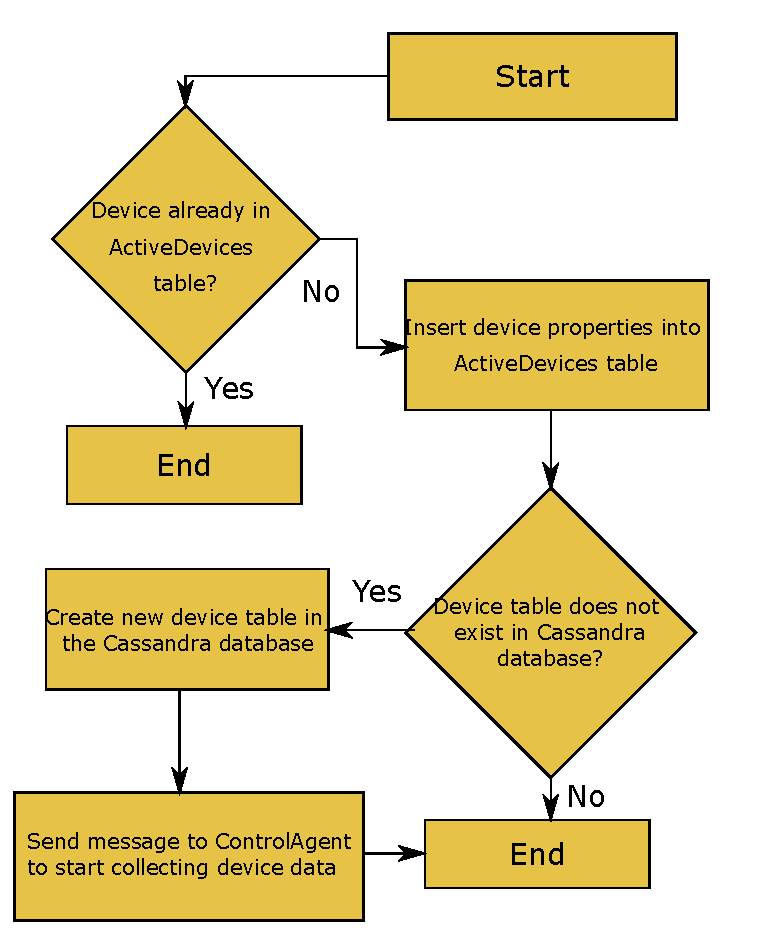
\includegraphics[scale=0.35]{figs/agents/setDeviceToActiveFlow.pdf}
        \caption{\texttt{DiscoveryAgent.setDeviceToActive()} flow chart}
        \label{fig:setDeviceToActiveFlow}
    \end{figure}
\end{frame}

\begin{frame}{Preliminary Work - Design}{}
    \begin{figure}
        \centering
        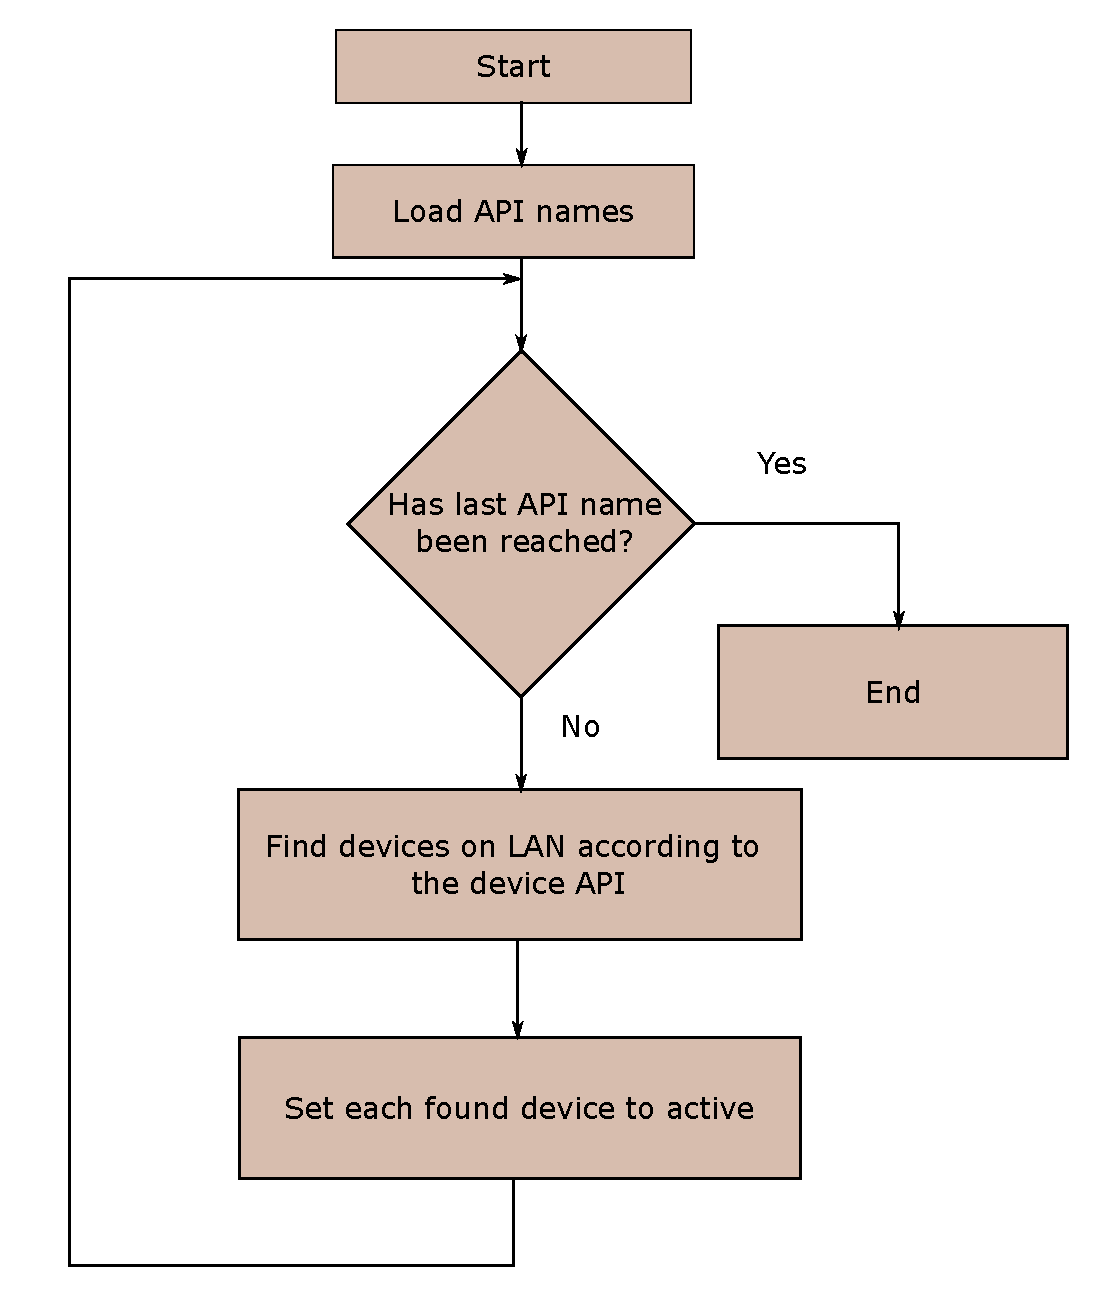
\includegraphics[scale=0.3]{figs/agents/searchForDevicesFlow.pdf}
        \caption{\texttt{DiscoveryAgent.searchForDevices()} flow chart}
        \label{fig:searchForDevicesFlow}
    \end{figure}
\end{frame}

\begin{frame}{Preliminary Work - Design}{}
    \begin{figure}
        \centering
        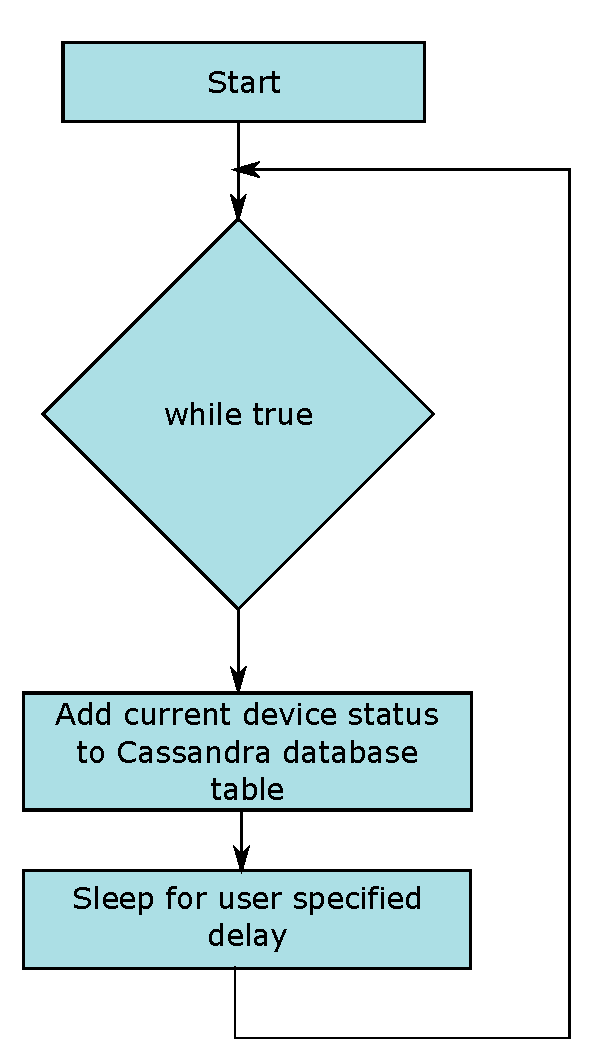
\includegraphics[scale=0.3]{figs/agents/periodicQueryBehaviorFlow.pdf}
        \caption{\texttt{ControlAgent.periodicQueryBehavior()} flow chart}
        \label{fig:periodicQueryBehavior}
    \end{figure}
\end{frame}

\begin{frame}{Device APIs}
    \begin{itemize}
        \item setState - Setter for Wemo Insight Switch and motor controllers on Embedded Computer
        \item getState - Returns power usage and on/off status for Wemo Insight Switch and PWM setting for Embedded Computer
        \item findDevices - Returns IP address of supported devices on the network
        \item findMetadata - Returns manufacturer, name, and MAC address of supported devices
        \item For Wemo Insight Switch, IP multicasting and Universal Plug and Play are used to send messages
        \item We are using a Beaglebone Blue for an embedded computer and so far have only used IP multicasting for communication
    \end{itemize}
\end{frame}

\begin{frame}{Experimental Setup}
    \begin{figure}
        \centering
        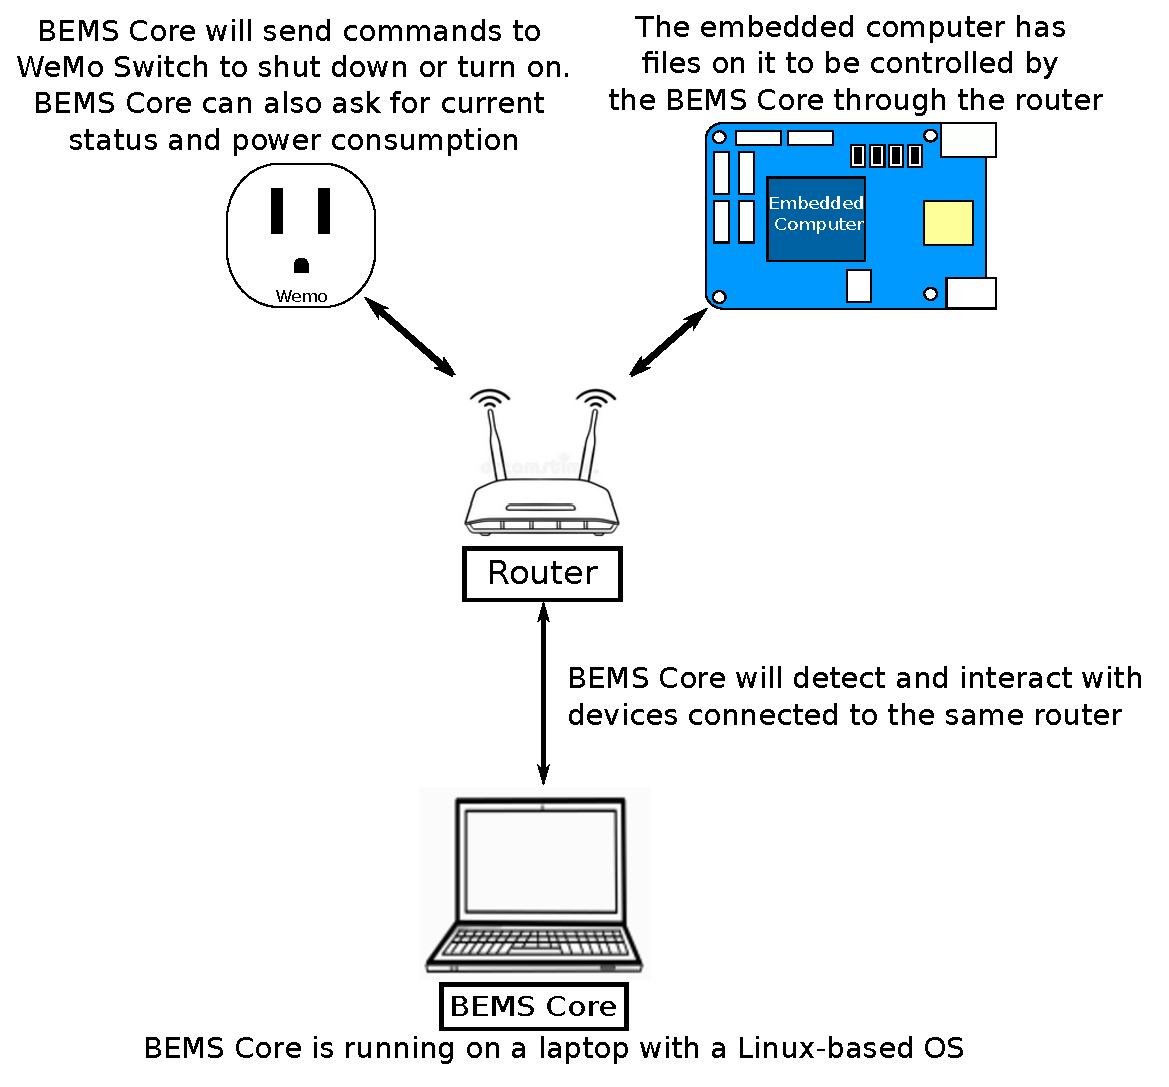
\includegraphics[scale=0.3]{figs/experimentalSetup.pdf}
        \caption{Lab Setup for Testing and Development}
        \label{fig:my_label}
    \end{figure}
\end{frame}

\begin{frame}{Preliminary Work - Experimental Activities}{}
    \begin{figure}
        \centering
        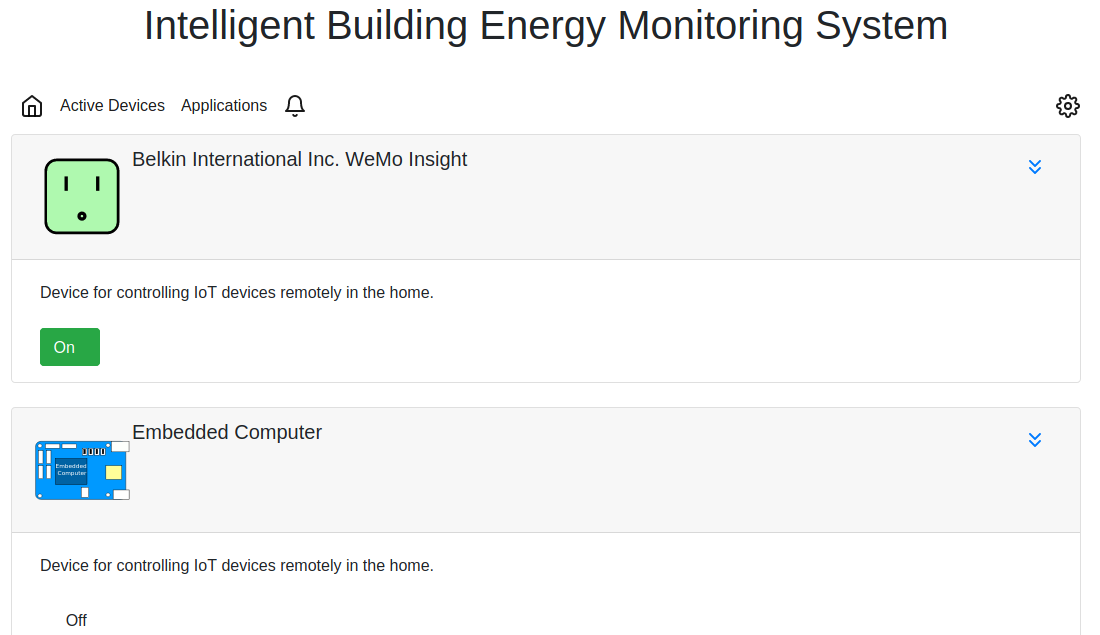
\includegraphics[scale=0.3]{figs/webServer/activeDevicesWithEmbeddedPicture.png}
        \caption{Screenshot of Web Server (Active Devices Page)}
        \label{fig:my_label}
    \end{figure}
\end{frame}

\begin{frame}{Preliminary Work - Experimental Activities}{}
    \begin{figure}
        \centering
        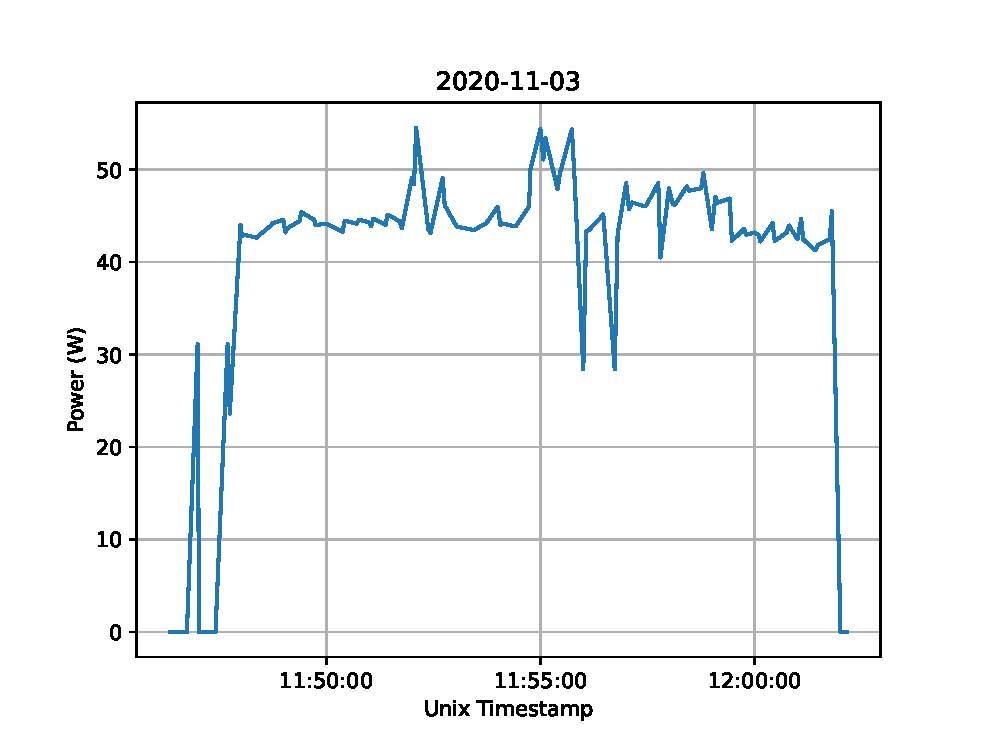
\includegraphics[scale=0.5]{figs/powerPlot2020-11-03.eps}
        \caption{Plot of WeMo Switch power usage 2020-11-03}
        \label{fig:powerPlotWeMoSwitch}
    \end{figure}
\end{frame}

\begin{frame}{Preliminary Work - Experimental Activities}{}
    \begin{itemize}
        \item Up to this point, work has been completed on the web user interface which was developed with the Bootstrap CSS framework and the JQuery Javascript framework
        \item When a request is sent to the active devices URL, the discovery agent will ping all possible supported devices on the network and newly discovered devices will appear on the active devices page
        \item the refresh button will cause the position of the slide switch switch shown to change depending on whether the WeMo switch is on or off
        \item The top nav bar will link to other pages including the home page, applications page, notifications and settings page (active devices is currently the only page implemented)
    \end{itemize}
\end{frame}

\begin{frame}{Parts List}{}
    \begin{itemize}
        \item WeMo Insight Smart Plug
        \item BeagleBone Blue
        \begin{itemize}
            \item Octavo OSD3358 Microprocessor
            \item Wifi/Bluetooth
            \item IMU/Barometer
            \item Power Regulation and state-of-charge LEDs for a 2-cell LiPo
            \item H-Bridges
            \item Connectors for 4 DC motors and 8 Servos
        \end{itemize}
        \item JST-ZH connector (for BeagleBone Blue Motor Connections)
        \item DC Motor
        \item ECE department laptop
        \item ECE department lab computers
    \end{itemize}
\end{frame}
% https://www.lucidchart.com/pages/templates/network-diagram
\begin{frame}{Timeline and Milestones}
\begin{ganttchart}[
hgrid,vgrid,x unit=.55cm, y unit title=.6cm,y unit chart=.4cm,milestone label font=\tiny,bar label font=\tiny, group label font=\small,bar/.append style={fill=green},bar incomplete/.append style={fill=red}]{3}{16}
\gantttitle{Fall 2020}{14}\\
\gantttitle{Sep}{2}
\gantttitle{Oct}{4}
\gantttitle{Nov}{4}
\gantttitle{Dec}{4}\\
\ganttgroup[progress = 100,group progress label font = \tiny,group progress label anchor = east]{WeMo Functionality}{3}{5} \\
\ganttbar[progress = 100,bar progress label font = \tiny,bar progress label anchor = east]{Refresh Status on Web Server}{3}{5}\\
\ganttbar[progress = 100,bar progress label font = \tiny, bar progress label anchor = east]{Record Power Usage}{3}{5}\\
\ganttgroup[progress = 67,group progress label font = \tiny,group progress label anchor = east]{Data Logging Feature}{5}{10}\\
\ganttbar[progress = 80,bar progress label font = \tiny,bar progress label anchor = east]{Support for Cassandra database}{5}{9}\\
\ganttbar[progress = 0,bar progress label font = \tiny,bar progress label anchor = east]{Matplotlib Plot in UI}{10}{10}\\
\ganttgroup[progress = 0,group progress label font = \tiny, group progress label anchor = east]{User Login}{11}{14}\\
\ganttbar[progress = 0,bar progress label font = \tiny,bar progress label anchor = east]{Login Page}{11}{12}\\
\ganttbar[progress = 0,bar progress label font = \tiny,bar progress label anchor = east]{Session Management}{13}{14}\\
\ganttgroup[progress = 55,group progress label font = \tiny,group progress label anchor = east]{Embedded Computer Functionality}{7}{14}\\
\ganttbar[progress = 90,bar progress label font = \tiny,bar progress label anchor = east]{Communication with BEMS}{7}{11}\\
\ganttbar[progress = 0,bar progress label font = \tiny,bar progress label anchor = east]{PWM Motor Control}{12}{13}\\
\ganttbar[progress = 0,bar progress label font = \tiny,bar progress label anchor = east]{Record Power Usage}{14}{14}
\end{ganttchart}
\end{frame}

\begin{frame}{Timeline and Milestones}
\begin{ganttchart}[
hgrid,vgrid,x unit=.45cm, y unit title=.6cm,y unit chart=.4cm,milestone label font=\tiny,bar label font=\tiny, group label font=\small,bar/.append style={fill=green},bar incomplete/.append style={fill=red}]{3}{16}
\gantttitle{Spring 2021}{14}\\
\gantttitle{Jan}{2}
\gantttitle{Feb}{4}
\gantttitle{Mar}{4}
\gantttitle{Apr}{4}\\
\ganttgroup[progress = 0,group progress label font = \tiny, group progress label anchor = east]{Simscape Microgrid}{3}{8}\\
\ganttbar[progress = 0,bar progress label font = \tiny,group progress label anchor = east]{Setup Simscape Microgrid}{3}{5}\\
\ganttbar[progress = 0,bar progress label font = \tiny,group progress label anchor = east]{Get Power Meter Data}{6}{8}\\
\ganttgroup[progress = 0,group progress label font = \tiny,group progress label anchor = east]{HVAC Control}{9}{14} \\
\ganttbar[progress = 0,bar progress label font = \tiny,bar progress label anchor = east]{Create HVAC system in Simscape}{9}{11} \\
\ganttbar[progress = 0,bar progress label font = \tiny,bar progress label anchor = east]{Implement LQR Algorithm for HVAC Control}{12}{14} \\
\ganttgroup[progress=0,group progress label font=\tiny,group progress label anchor = east]{Auto Discovery}{15}{16}\\
\ganttgroup[progress = 0,group progress label font = \tiny,group progress label anchor = east]{Weather Service Update}{15}{16}\\
\ganttbar[progress = 0,bar progress label font = \tiny,group progress label anchor = east]{Receive Weather Data}{15}{15}\\
\ganttbar[progress = 0,bar progress label font = \tiny,group progress label anchor = east]{Display Notification}{16}{16}
\end{ganttchart}    
\end{frame}

% \begin{frame}{Timeline and Milestone}
% \begin{ganttchart}[
% hgrid,vgrid,x unit=.55cm, y unit title=.6cm,y unit chart=.4cm,milestone label font=\tiny,bar label font=\tiny, group label font=\small,bar/.append style={fill=green},bar incomplete/.append style={fill=red}]{1}{18}

% \end{ganttchart}    
% \end{frame}

% You can reveal the parts of a slide one at a time
% with the \pause command:
%\begin{frame}{Second Slide Title}
%  \begin{itemize}
%  \item {
%    First item.
%    \pause % The slide will pause after showing the first item
%  }
  %\item {   
  %  Second item.
 % }
  % You can also specify when the content should appear
  % by using <n->:
 % \item<3-> {
 %   Third item.
 % }
%  \item<4-> {
%    Fourth item.
 % }
  % or you can use the \uncover command to reveal general
  % content (not just \items):
%  \item<5-> {
%    Fifth item. \uncover<6->{Extra text in the fifth item.}
%  }
%  \end{itemize}
%\end{frame}

%\section{Second Main Section}

% \subsection{Another Subsection}

% \begin{frame}{Blocks}
% \begin{block}{Block Title}
% You can also highlight sections of your %presentation in a block, with it's own %title
% \end{block}
% \begin{theorem}
% There are separate environments for %theorems, examples, definitions and proofs.
% \end{theorem}
% \begin{example}
% Here is an example of an example block.
% \end{example}
% \end{frame}

% Placing a * after \section means it will not show in the
% outline or table of contents.
\section*{Summary}
\begin{frame}{Summary} %Brian
  \begin{itemize}
    \item Development of a platform to control devices
    \item Ability to read device status (power usage, state)
    \item Smart grid simulation using Simscape and Matlab
    \item HVAC control algorithm using Linear Quadratic Regulator (LQR)
  \end{itemize}
\end{frame}
% \begin{frame}{Summary}
%   \begin{itemize}
%   \item
%     The \alert{first main message} of your talk in one or two lines.
%   \item
%     The \alert{second main message} of your talk in one or two lines.
%   \item
%     Perhaps a \alert{third message}, but not more than that.
%   \end{itemize}
  
%   \begin{itemize}
%   \item
%     Outlook
%     \begin{itemize}
%     \item
%       Something you haven't solved.
%     \item
%       Something else you haven't solved.
%     \end{itemize}
%   \end{itemize}
% \end{frame}



% All of the following is optional and typically not needed. 
\appendix
\section<presentation>*{\appendixname}
\subsection<presentation>*{For Further Reading}

\begin{frame}[allowframebreaks]
  \frametitle<presentation>{References}
    
  \begin{thebibliography}{10}
    
  \setbeamertemplate{bibliography item}[online]
  
  \bibitem{bemoss}
  BEMOSS 3.5
  \newblock \url{https://github.com/bemoss/BEMOSS3.5}
  
  \bibitem{flask}
  Flask Documentation
  \newblock \url{https://flask.palletsprojects.com/en/1.1.x/}
  
  \bibitem{datastaxPython}
  Datastax Python 3 Cassandra Driver
  \newblock \url{https://docs.datastax.com/en/developer/python-driver/3.24/}
  
  \bibitem{apacheCassandra}
  Apache Cassandra Database
  \newblock \url{https://cassandra.apache.org/}
  \end{thebibliography}
\end{frame}

\begin{frame}{References}
    \bibliographystyle{IEEEtran}
    \bibliography{bib/references.bib}
\end{frame}

\end{document}



%%% Local Variables:
%%% mode: latex
%%% TeX-master: t
%%% End:
